\documentclass[12pt]{article}
\setlength\parindent{0pt}
\usepackage[left=1in, right=1in, top=0.65in, bottom=1.0in]{geometry}
\usepackage{graphicx}
\usepackage[utf8]{inputenc}
\usepackage{wrapfig}
\usepackage{geometry}
\usepackage{mathtools}

\usepackage{amsfonts, amsthm, amsmath, braket}
\usepackage{tikz}
\usetikzlibrary{angles, quotes,calc,patterns}
\usepackage{tikz}
\usetikzlibrary{positioning}

\usepackage{pgfplots}
\usepgfplotslibrary{polar}
\pgfplotsset{compat=1.10}

\renewcommand{\baselinestretch}{1.0}
\setlength{\parskip}{0.5em}


\title{Ionsonde Antenna Calculations \vspace{-2ex}}
\author{Blair3Sat}
\date{}

\begin{document}
\maketitle

\section*{Introduction}
The goal of this project is simply to generate a function for the power received by an antenna as a function of the size and antenna and the location/position of the cube satellite. 
\subsection*{Background}
Before calculating the power that an antenna will receive, it is important to understand the two antennas being analyzed. First, the transmitter is the VIPIR ionosonde chirper at Wallops, VA. Our goal is to simulate the necessary antenna length for an antenna receiving an ionosonde at $30^\circ$ from 408 km above the earth's surface.

\subsection*{Calculations}
\begin{figure}[h]
\centering
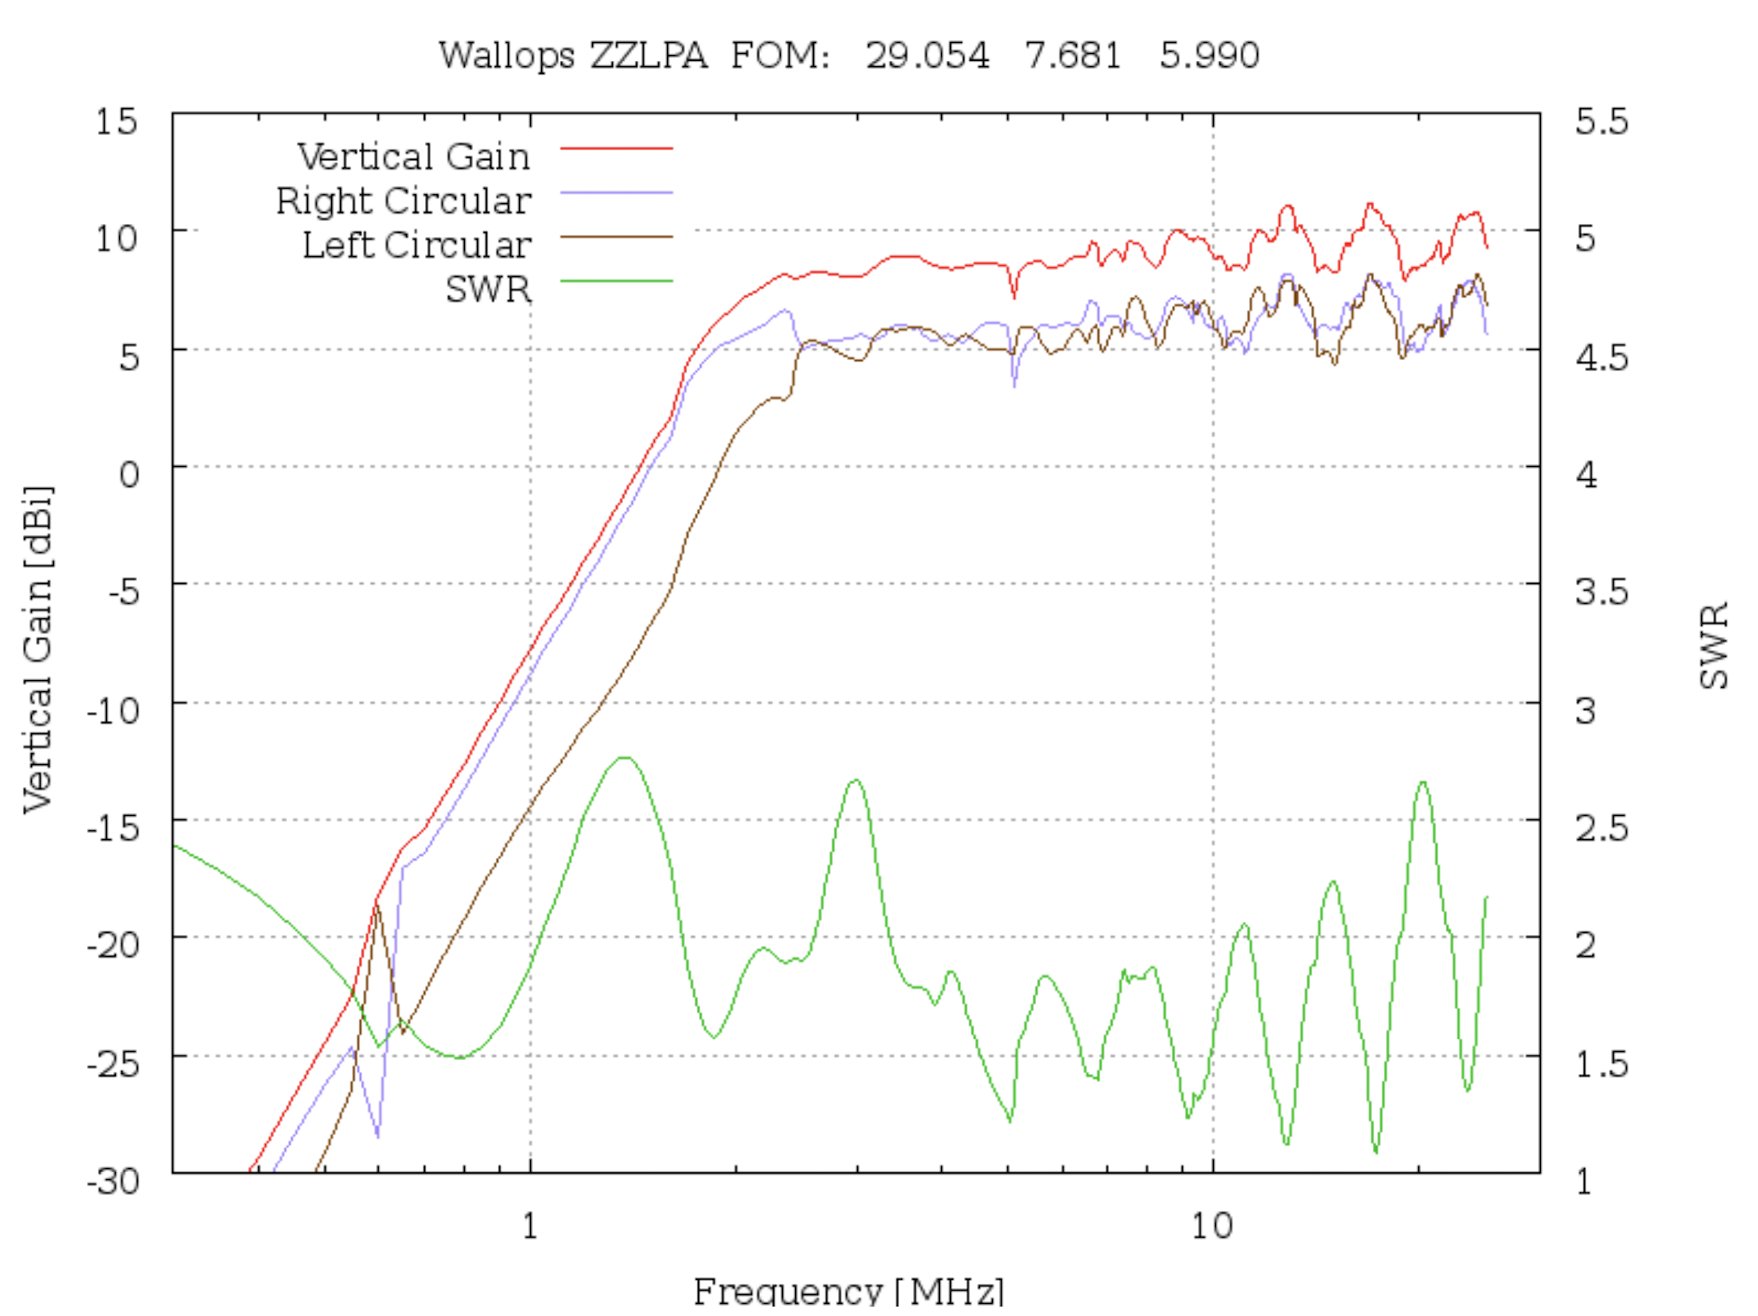
\includegraphics[width=0.8\textwidth]{vipir_one}
\caption[Caption for LOF]{Measured ionosonde gain and SWR\protect\footnotemark}
\label{fig:swr}
\end{figure}

Let's start with what's needed to calculate power. The basic formula for power transmitted to an antenna is as follows:
 $$
 P_{rx} = P_{tx}G_{tx}G_{rx} \Bigg( \frac{c}{4\pi D_r f_0} \Bigg)^2
 $$
 
$P_{tx}$ represents from the power from the transmitting antenna and can currently be estimated to be 20 watts and considering the effect of VSWR becomes $88.9 \%$ of that or 17.78. The gain of the antenna is given by  the following chart produced by the VIPIR team [\ref{fig:swr}]. The gain on average for the range 2-20 MHz is roughly 7 dBi, but can be under-approximated to 5 dBi.

In order to model the power of the antenna at different angles we will use the diagram provided by the VIPIR team [\ref{fig:angle}]. 

\begin{figure}[h]
\centering
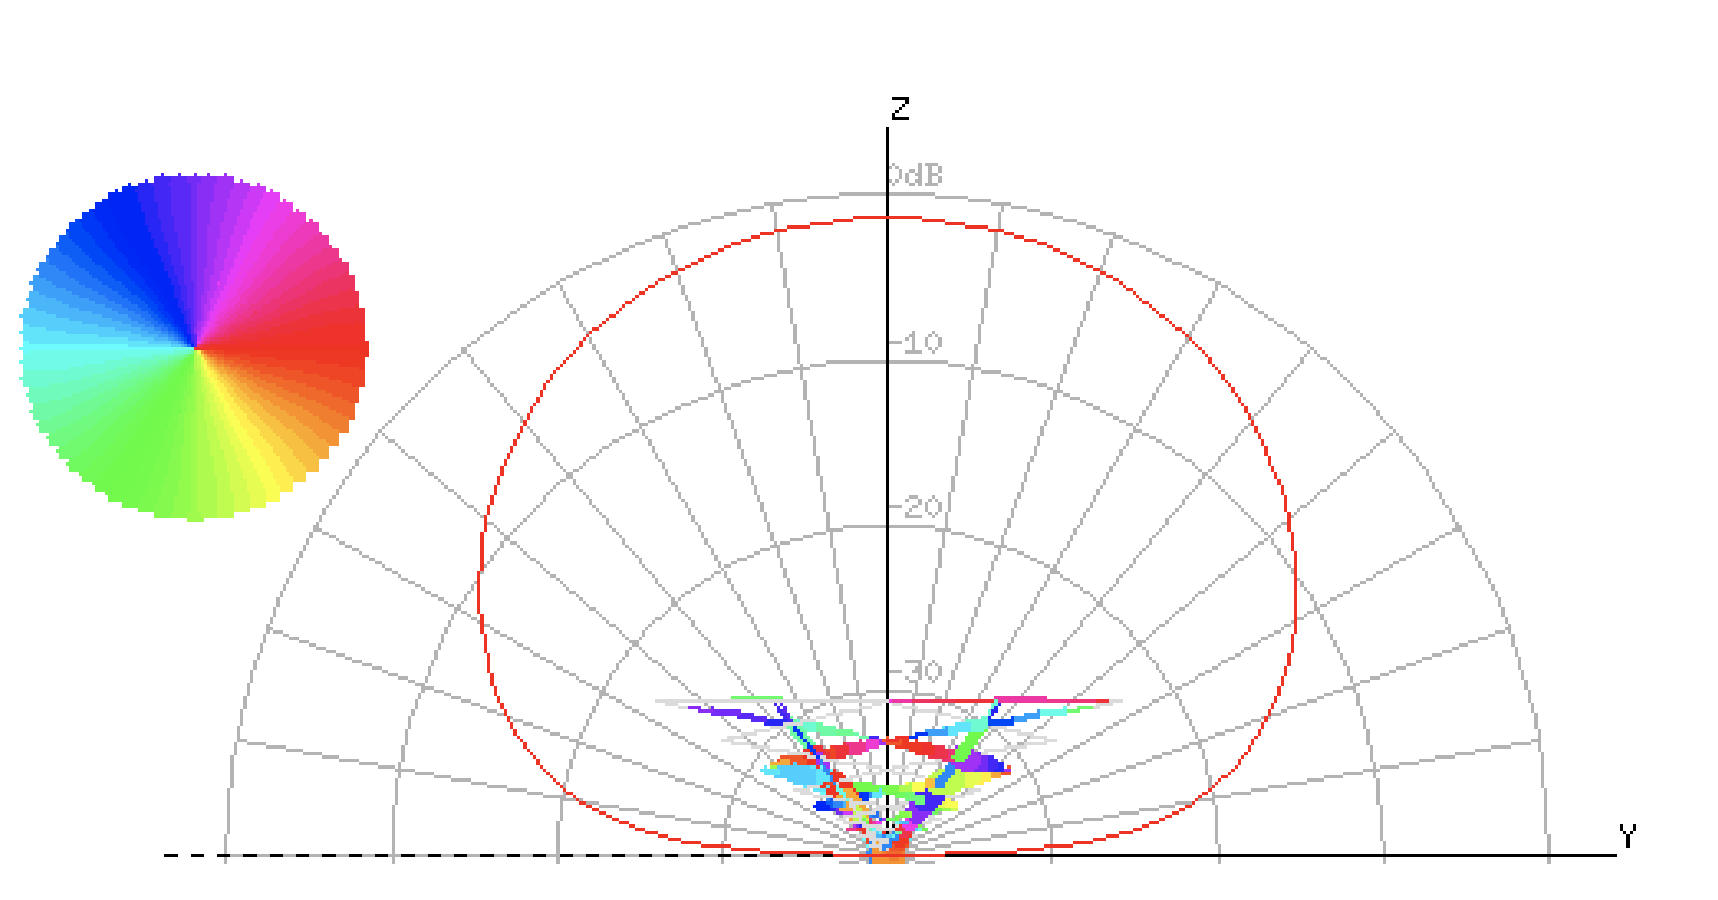
\includegraphics[width=0.65\textwidth]{vipir_two}
\caption[Caption for LOF]{Measured ionosonde gain at different angles\protect$^1$}
\label{fig:angle}
\end{figure}
The exact equation is not provided by the team so instead, we will model the gain using a piecewise made by connecting the points observed in the photo above. We start with collecting all the points $r_n$ and $\theta_n$ and converting this set of points to coordinate axis points. From there, any given angle is converted to the equation $y = \tan(\theta_i)x$ and the intercept is found with $y = \big( \frac{y_2-y_1}{x_2-x_1} \big)x+b$. We will denote the gain of this antenna at any angle as $G(\theta_1)$. $\theta_1$ being the angle from the latitude and longitude of the ground station to the current antenna position.


\footnotetext{http://www.ursi.org/proceedings/procGA08/papers/GP2GHp3.pdf}

For the gain of a lossless short dipole is: $$G(\theta_1)=1.5\sin^2(\theta_2)$$

where A is the distance between the center of the earth and B is the radius of the earth:

$$
\theta_1 = 180 - \theta_2  - \arcsin \Big( \frac{A \sin(\theta_2)}{B} \Big)
$$



\newpage

$\theta_1$ relates to $\theta_2$ as shown below:

\begin{center}

\tikzset{every picture/.style={line width=0.75pt}} %set default line width to 0.75pt        

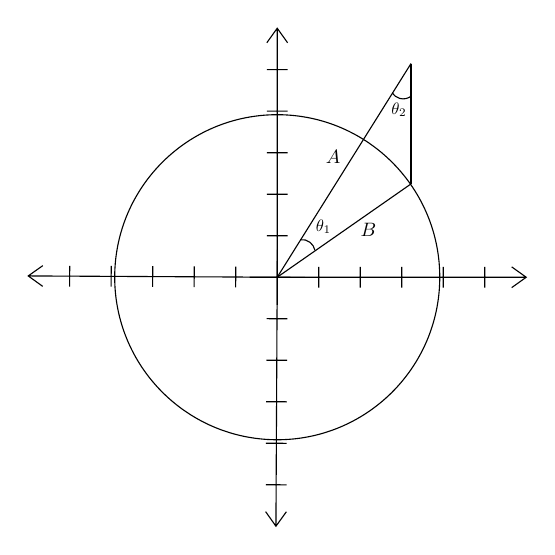
\begin{tikzpicture}[x=0.75pt,y=0.75pt,yscale=-1,xscale=1]
%uncomment if require: \path (0,300); %set diagram left start at 0, and has height of 300

%Shape: Axis 2D [id:dp7363032892918209] 
\draw  (242.7,162.97) -- (376,162.97)(256.03,43) -- (256.03,176.3) (369,157.97) -- (376,162.97) -- (369,167.97) (251.03,50) -- (256.03,43) -- (261.03,50) (276.03,157.97) -- (276.03,167.97)(296.03,157.97) -- (296.03,167.97)(316.03,157.97) -- (316.03,167.97)(336.03,157.97) -- (336.03,167.97)(356.03,157.97) -- (356.03,167.97)(251.03,142.97) -- (261.03,142.97)(251.03,122.97) -- (261.03,122.97)(251.03,102.97) -- (261.03,102.97)(251.03,82.97) -- (261.03,82.97)(251.03,62.97) -- (261.03,62.97) ;
\draw   ;
%Shape: Axis 2D [id:dp8361304849729825] 
\draw  (269.36,163.04) -- (136.07,162.34)(255.41,282.93) -- (256.1,149.64) (143.04,167.37) -- (136.07,162.34) -- (143.1,157.37) (260.44,275.96) -- (255.41,282.93) -- (250.44,275.9) (236.01,167.86) -- (236.06,157.86)(216.01,167.76) -- (216.06,157.76)(196.01,167.65) -- (196.06,157.65)(176.01,167.55) -- (176.06,157.55)(156.01,167.44) -- (156.06,157.44)(260.93,182.99) -- (250.93,182.94)(260.82,202.99) -- (250.82,202.94)(260.72,222.99) -- (250.72,222.94)(260.62,242.99) -- (250.62,242.94)(260.51,262.99) -- (250.51,262.94) ;
\draw   ;
%Shape: Ellipse [id:dp5110872767224213] 
\draw   (177.73,162.38) .. controls (178.06,119.13) and (213.38,84.34) .. (256.62,84.66) .. controls (299.87,84.99) and (334.66,120.31) .. (334.34,163.55) .. controls (334.01,206.8) and (298.69,241.59) .. (255.45,241.27) .. controls (212.2,240.94) and (177.41,205.62) .. (177.73,162.38) -- cycle ;
%Straight Lines [id:da09325332790069751] 
\draw    (256.03,162.97) -- (320.5,60) ;


%Straight Lines [id:da3268485149219602] 
\draw    (256.03,162.97) -- (320.5,118) ;


%Straight Lines [id:da4332191392765037] 
\draw    (320.5,118) -- (320.5,60) ;


%Shape: Arc [id:dp16308496569160624] 
\draw  [draw opacity=0] (267.07,144.91) .. controls (268.7,144.67) and (270.41,145.05) .. (271.8,146.11) .. controls (273.08,147.08) and (273.88,148.46) .. (274.17,149.94) -- (267.8,151.38) -- cycle ; \draw   (267.07,144.91) .. controls (268.7,144.67) and (270.41,145.05) .. (271.8,146.11) .. controls (273.08,147.08) and (273.88,148.46) .. (274.17,149.94) ;
%Shape: Arc [id:dp5617692644110672] 
\draw  [draw opacity=0] (320.53,75.75) .. controls (319.01,76.89) and (317.03,77.35) .. (315.09,76.83) .. controls (313.54,76.41) and (312.28,75.45) .. (311.45,74.18) -- (316.8,70.44) -- cycle ; \draw   (320.53,75.75) .. controls (319.01,76.89) and (317.03,77.35) .. (315.09,76.83) .. controls (313.54,76.41) and (312.28,75.45) .. (311.45,74.18) ;

% Text Node
\draw (278.33,138.67) node [scale=0.6]  {$\theta _{1}$};
% Text Node
\draw (314.67,82.33) node [scale=0.6]  {$\theta _{2}$};
% Text Node
\draw (283,105) node [scale=0.7]  {$A$};
% Text Node
\draw (300,140) node [scale=0.7]  {$B$};


        
\end{tikzpicture}
\end{center}

At $30^o$ the gain value is 1.125. Plugging all known values back into Friis's equation we get 8.303e-10 W as the power received at the antenna.



The input impedance of the antenna is:
$$
Z = R_{rad} + R_{loss} +jX
$$ 

Radiation resistance is given by:
$$
R_{rad} = 20\pi^2 \Big( \frac{L}{\lambda} \Big)^2
$$

And radiation loss is given by:
$$
R_{loss} = \frac{L}{6\pi\alpha}\sqrt{\frac{\pi f \mu}{2 \sigma}}
$$

where $\sigma$ is the conductivity of the dipole.

The imaginary part of the dipole is given by:
$$
X = \frac{-120\lambda}{\pi L} \Big( \ln \frac{L}{2 \alpha} - 1 \Big)
$$

Thus for antenna that we consider to have the radius of 5mm and a length of 1m, where the antenna operates at a frequency of 15MHz and using titanium as the metal with a conductivity of $2.38 \cdot 10^6\:S/m$. The radiation resistance is calculated to be 0.39 Ohms. The loss resistance is 5.51 mOhms, and the imaginary part is ~1500 Ohms. Calculated VSWR is 1.28.

This finally gives us a received power of $98 \%$ the final power or 8.13694e-10 W.

\newpage


\end{document}
